\documentclass[a4paper,12pt]{article}
\usepackage[french,english]{babel}
\usepackage[utf8x]{inputenc}
\usepackage{graphicx}
\usepackage{tikz,pgfplots}
\usepackage{setspace}
\usepackage{abstract}
\usepackage[T1]{fontenc}
\usepackage[top=2.8cm, bottom=2.8cm, left=3cm, right=3cm]{geometry}
\usepackage{subfig}
\usepackage{amsmath,amsfonts,amssymb,amsthm,mathtools,mathrsfs}
\usepackage{float}
\usepackage{enumerate}
\usepackage{unnumberedtotoc}
\usepackage[justification=centering]{caption}
\usepackage{hyperref}
\usepackage{stmaryrd}
\usepackage{algpseudocode}
\usepackage{algorithm}
\usepackage{algorithmicx}
\usepackage{indentfirst}


% Keywords command
\providecommand{\keywords}[1]
{
  %\small    
  \textbf{\textit{Keywords---}} #1
}


\title{SPOT: Sliced Partial Optimal Transport}
%\author{effaitunail}
%\date{May 2018}

\begin{document}

%-----------------------------Title-Page-------------------------------

\begin{titlepage}
\begin{center}


\includegraphics[scale=0.7]{ENPC.png}

\includegraphics[scale=0.25]{ENS.png}

\textsc{\Large }\\[1cm]

% Title
\rule[5pt]{\linewidth}{.7pt}

{\huge \bfseries \textsc{SPOT: Sliced Partial Optimal Transport  \\-\\ fast python implementation, Color transfer, and point cloud registration\\[0.4cm] }}

\rule[5pt]{\linewidth}{.7pt}

% Author 
\emph{Auteur:}\\
Quentin \textsc{Spinat}


\vfill

% Bottom of the page
{\large \today}

\end{center}
\end{titlepage}

%-----------------table-des-matières------------------------

\tableofcontents
\thispagestyle{empty}
\setcounter{page}{0}

\newpage

%---------------------Abstract-en-une-seule-colonne--------------------

\begin{center}
\textbf{Abstract}
\end{center}

This is paper is the project report for the 2020 MVA course \textit{Computational Optimal Transport} taught by Gabriel Peyré. The purpose of it is to study the paper \textit{SPOT: Sliced Partial Optimal Transport} \cite{BC19}.

Optimal Transport is a mathematical field that focus on finding the best way to match two sets with respect to a matching cost. Here we will focus on a subproblem which consists in finding the best injective assignment of a finite set of points to a second bigger set of points. Although it is a very precise problem, it is often encountered : color transfer from an Image to a bigger one, matching a small point clouds to a bigger one, ...

Nicolas Bonneel et al. proposed a method they called FIST : Fast Iterative Sliced Transport to solve this problem. It consists in solving the assignment problem considering only 1D optimal assignments, which are fast and easy to compute. Their algorithm is told to be quasilinear in time with respect to the datasets sizes.

In this project, I clarify the explanations of the original paper (which is full of typos, especially in the algorithm description), make a fast and user-friendly implementation of this algorithm in Python, and apply it to color transfer and point cloud registration.

Even though I wasn't able to parallelize my code due to python limitations, the implementation I made revealed to be faster than the original implementation in C\texttt{++} for color transfer application. However I couldn't be able to reproduce good results for point cloud registration.

\bigskip

%\vfill % ou \hspace{10pt} ??

\keywords{Optimal Transport, Optimal assignment, SGD, Shape matching, Color transfer}

\begin{center}
    \rule{4cm}{0.4pt}
\end{center}


%---------------------------Corps-------------------------------

\bigskip

\addsec{Introduction}
%\section*{Introduction}

\subsection*{Problem}

Optimal Transport is a mathematical field that focus on finding the best way to match two sets with respect to a matching cost. Here we will focus on a subproblem which consists in finding the best injective assignment of a finite set of points to a second bigger set of points. Although it is a very precise problem, it is often encountered : color transfer from an Image to a bigger one, matching a small point clouds to a bigger one. 

\subsubsection*{Previous Work}

Optimal transport is a computationally complex problem, often expressed as a linear program due to Kantorovich. The variables being optimized form what is known as a transport plan to describe the amount of mass from each bin of an input (possibly high-dimensional) histogram that needs to travel to each bin of a target histogram. In this definition, it is assumed that both histograms are normalized. Directly solving this linear program can be very costly in time and memory, and when dealing with a large amount of points, algorithms become very greedy, especially because of the curse of dimensionality. Faster alternate approaches have been developed to tackle particular cases, but cannot be applied to the problem we try to overcome.

This is why the field of sliced optimal transport has emerged. It consists in projecting the point clouds onto random one-dimensional subspaces, and solving one-dimensional transport problems [Pitie et al. Rabin et al. \cite{pitie2005n}, Bonneel et al. \cite{rabin2011wasserstein}, \cite{bonneel2015sliced}]. Slicing methods are very fast because of how simpler one-dimensional optimal transport is to solve. However, Sliced optimal transport is only an approximation and comes at the cost of being optimal only on the projections and not necessarily on the higher dimensional space.
  But optimal transport for non-normalized histograms has received little attention, even in one-dimension, which makes the sliced approach not possible for point clouds of different sizes yet.
 
When histograms are not normalized, the transport problem needs to be relaxed. Notably, the "unbalanced" optimal transport of Benamou et al. \cite{benamou2003numerical} replaces hard constraints by soft constraints in a Monge formulation to accommodate for densities of unequal masses within a PDE framework. However, it suffers from a big space complexity. Figalli introduces \textit{partial optimal transport} that keeps all constraints of the linear program hard \cite{figalli2010optimal}, but replaces equality with inequality constraints. The problem we are interested in is a special case of this linear program for the problem of matching point clouds.

\subsubsection*{New Contributions}

Nicolas Bonneel et al. \cite{BC19} proposed a Sliced Partial Optimal Transport (SPOT) method they called FIST : Fast Iterative Sliced Transport to solve the problem of optimal injective assignment between point clouds of different sizes. This is a sliced method which consists in minimizing the mean over all the one-dimensional projections of the Wassertein distance between the two 1D projected point clouds. It hence makes it possible to solve the original problem by doing a Stochastic Gradient Descent and solving only the 1D projected subproblems.
To solve these one-dimensional partial optimal transport subproblems efficiently, they propose an algorithm quasilinear in time with respect to the datasets sizes.

\subsection*{Applications}

In this project, we focus on two applications of this new method : color transfer problem and point cloud registration.

\subsubsection*{Color Transfer}

Transferring colors between images has become a classical image processing problem. The purpose is to change the color distribution of an input image, without changing its content, to match the style of a target image. Numerous optimal transport solutions have already been developed [Bonneel et al. \cite{bonneel2015sliced}, \cite{bonneel2013example}; Pitié et al. \cite{pitie2005n}; Pitié et al. \cite{pitie2007automated}; Rabin et al. \cite{rabin2010regularization}]. In addition to their use of optimal transport, a common point to these approaches is that they consider the problem of matching normalized histograms. A consequence of that is often acknowledged as a limitation: their content should not differ. For instance, matching an image with 80\% trees and 20\% sky to an image containing the opposite ratio will inevitably lead to trees becoming blue or sky becoming green. Several approaches also require the images to have exactly the same number of pixels – this is precisely the case for sliced transportation [Bonneel et al. \cite{bonneel2015sliced}; Rabin et al. \cite{rabin2010regularization}].

Bonneel et al. proposed two solutions to overcome these problems, but I only focus on one of them : this solution simply enlarges the target images to give more freedom to each input pixel to be matched to target pixel values. This method is really fast and produces really good results

\subsubsection*{Point Cloud Registration}

A common problem in point cloud processing is that of registering points under a given transformation model. For instance, one tries to match a point cloud with another by supposing the transformation between them is rigid, or constrained to a similarity, or affine, or homographic, etc. A well-known algorithm to solve this problem is the Iterative Closest Point (ICP) algorithm. Given a point cloud $X_0$ to be matched against $X_1$ , this algorithm proceeds by first matching points of $X_0$ to their nearest neighbors in $X_1$ , and, given this assignment, the best transformation in the class of allowed transformations is found by minimizing an energy. The algorithm then transforms the initial point cloud using the computed transformation. The process is repeated until convergence. However, this algorithm requires points clouds to be relatively close to start with and suffers from local minima. In practice, extremely bad behaviors may arise when considering similarity transforms (rotation, translation and scaling). In that case, the lack of injectivity of the nearest neighbor map tends to estimate progressively smaller scaling factors as iterations increase, occasionally leading to a trivial zero scale solution.

This motivates the use of a metric which accounts for an injective mapping, such as the sliced metric proposed by Bonneel et al. They thus propose to replace the nearest neighbor matching by a partial sliced optimal transport matching they call \textit{Fast Iterative Sliced Transport} (FIST). 


\newpage

\section{Partial Transport in 1-D}

This section will explain the core of this new method, which is an efficient algorithm for Partial Transport in one dimension. It relies on the fact that the nearest neighbor assignment of two point sets can be found in linear time in one-dimension. However, this nearest neighbor assignment not being injective. However, we need to smartly modify it. This can easily be done in quadratic time. To go further and improve the algorithm performances, we need then to introduce a way to decompose the original problem into independent easier problems, which can be solved in parallel. With this problem decomposition, the whole algorithm becomes quasilinear in time.

In all the problem we consider that $X$ is a set of 1-D points of cardinal $m$, $Y$ a set of 1-D points of cardinal $n<m$, and that $X$ and $Y$ are sorted by increasing value (this can be done in quasilinear time). We also write $\alpha = \dfrac{m}{n}$.

\subsection{Nearest Neighbor Assignment}

In one dimension, the nearest neighbor assignment $t : \llbracket 1,m \rrbracket \rightarrow \llbracket 1,n \rrbracket$ from $X$ to $Y$ can be found in linear time. Since $t(i) \leqslant t(i+1)$, the algorithm consists in scanning $X$ and $Y$ simultaneously from left to right and compare their value. \\

\begin{algorithm}
\caption{Nearest Neighbor Assignment}\label{t}
\hspace*{\algorithmicindent} \textbf{Input:} sorted $X,Y$\\
\hspace*{\algorithmicindent} \textbf{Output:} $t$ 
\begin{algorithmic}[1]
\State $i\gets 1$
\State $j\gets 1$
\While{$i<m$}
	\If{$x_i \leqslant y_j$}
		\State $t[i] \gets j$
		\State $i \gets i+1$
    \ElsIf {$j=n$}:
        \State $t[i] \gets n$
        \State $i \gets i+1$
    \ElsIf {$y_{j+1}<x_i$}
        \State $j \gets j+1$
    \ElsIf {$|x_i-y_j|<|x_i-y_{j+1}|$}:
        \State $t[i] \gets j$
        \State $i \gets i+1$
    \Else
        \State $t[i] \gets j+1$
        \State $j \gets j+1$
        \State $i \gets i+1$
    \EndIf
\EndWhile
\State \Return{$t$}
\end{algorithmic}
\end{algorithm}


\begin{figure}[H]
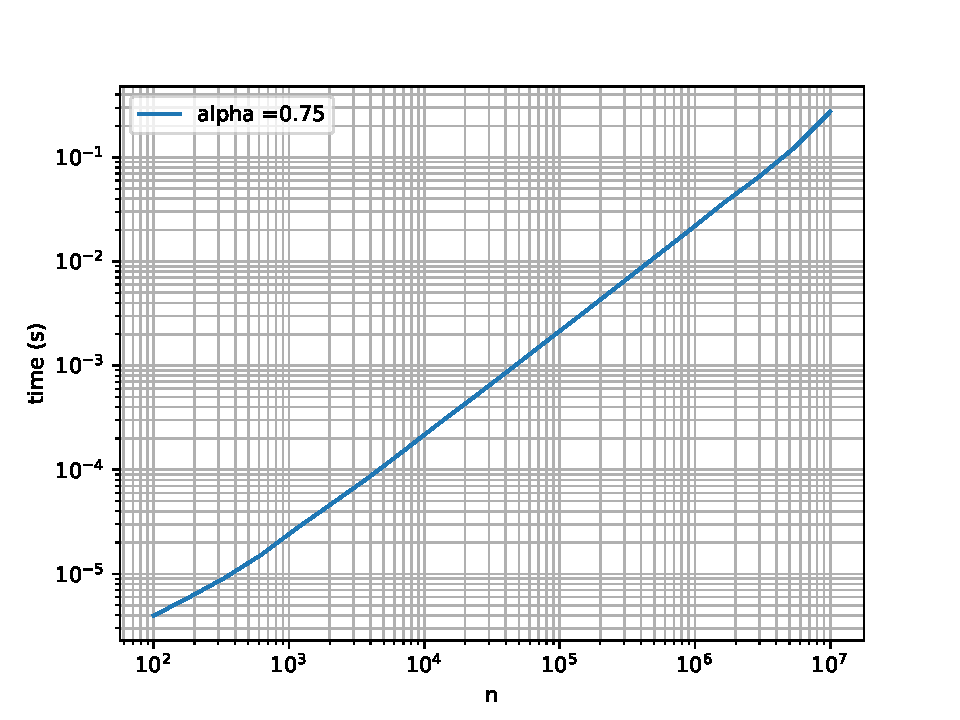
\includegraphics[width = \columnwidth]{t_time.pdf}
\caption{Mean time over $100$ simulations for Nearest Neighbor Assignment with respect to $n$, $\alpha=0.75$, logscale}\label{t_time}
\end{figure}

\subsection{Quadratic Time Algorithm}

As the nearest neighbor assignment may not be injective, we need to change it resolving issues around points where $t[i] = t[j]$ for $i \neq j$. To do so, we scan X from left to right and consider the sub-problem of matching $X' = \{x_i \}_{i \in \llbracket 1;m' \rrbracket} $ with $Y$ , progressively increasing $m'$ from $1$ to $m$. 

To create this assignment $a$ from $t$, we start by initializing $a[1] = t[1]$. Once $\{a[k]\}_{k \in \llbracket 0;i \rrbracket}$ is created, there is two options. If $t[i+1]>a[i]$, we put $a[i+1]=t[i+1]$. Else, there are two possible cases : we can either put $a[i+1]=a[i]+1$ (case 1), or put $a[i+1]=a[i]$ and translate every previous $a[k]$ from one to the left (case 2). The second option writes $ a[i+1] = a[i]$ and $a[r:i] = a[r:i]-1 $, where $r$ is such that $y_{a[r]-1}$ is the last available free spot of $Y$. We chose the solution that minimizes the distance between points (i.e $\sum_{k=1}^{i+1} (x_k - y_{a[k]})^2$). 

Proof that the partial assignment given by this algorithm is optimal is given in appendix \ref{a_quad_proof}.\\

\begin{algorithm}
\caption{Quadratic Partial Optimal Assignment}\label{a_quad}
\hspace*{\algorithmicindent} \textbf{Input:} sorted $X,Y$\\
\hspace*{\algorithmicindent} \textbf{Output:} $a$ 
\begin{algorithmic}[1]
\State compute $t$
\State $a[1] \gets t[1]$
\For{$i$ from $1$ to $m-1$}
	\If{$t[i+1] > a[i]$}
		\State $a[i+1] \gets t[i+1]$
		\State update $r$
    \Else
        \State $w_1 \gets \sum_{k=r}^{i} (x_k - y_{a[k]})^2 + (x_{i+1} - y_{a[i]+1})^2$
        \State $w_2 \gets \sum_{k=r}^{i} (x_k - y_{a[k]-1})^2 + (x_{i+1} - y_{a[i]})^2$
        \If {$w_1\leqslant w_2$} \Comment{Case 1}
        	\State $a[i+1] \gets a[i]+1$
        \Else \Comment{Case 2}
        	\State $a[i+1] \gets a[i]$
        	\State $a[r:i] \gets a[r:i]-1$
        	\State update $r$
        \EndIf
    \EndIf
\EndFor
\State \Return{$a$}
\end{algorithmic}
\end{algorithm}

This algorithm can be optimized to run faster. First, there trivial subcases :
\begin{itemize}
\item If $m=n$, we can directly put $a[i]=i$ for $i$ from $1$ to $m$.

\item If $m=n-1$, there exists some $k$ to be determined such that $a[1: k − 1] = [1: k − 1]$
and $a[k: m] = [k + 1: n]$. Such $k$ minimizes $\sum_{i=1}^{k-1} (x_i-y_i)^2 + \sum_{i=k}^{m} (x_i-y_{i+1})^2 $ . Denoting $C = \sum_{i=1}^m (x_i - y_{i+1})^2$, the above minimization problem can be written $\min_k \sum_{i=1}^{k-1} (x_i-y_i)^2 + C - (x i - y_{i+1})^2$ which can be obtained within a single linear search, as $C$ is a constant and need not be computed.

\item If $t$ is injective, we put $a=t$.
\end{itemize}

Second, we can simplify the problem before computing $a$.
\begin{itemize}
\item If there exists $i$ such that $X[1:i] \leqslant Y[1:i]$, we can put $a[1:i] = \llbracket 1;i \rrbracket$
\item If there exists $i$ such that $Y[i:n] \leqslant X[i:m]$, we can put $a[i:m] = \llbracket i;m \rrbracket$
\item If $p$ is the number of non-injective values of $t$, $p=card\{t[i] = t[i + 1], \forall i < m\}$, then, it is enough to consider the sub-problem of matching $X$ to $Y' = \{y_j\}_{j \in \llbracket max(1,t[1]−p) ; min(t[m]+p,n) \rrbracket}$
\end{itemize}

Finally, we don't have to re-evaluate the sums $w_1$ and $w_2$ each time. If we write $S_{i,1} = \sum_{k=r}^{i} (x_k - y_{a[k]})^2$ and $S_{i,2} = \sum_{k=r}^{i} (x_k - y_{a[k]-1})^2$, then in the loop $i$, we have $w_1 = S_{i,1} + (x_{i+1} - y_{a[i]+1})^2$ and $w_2 = S_{i,2} + (x_{i+1} - y_{a[i]})^2$. There is then three cases :
\begin{itemize}
\item If we put $a[i+1]>a[i]+1$, then $S_{i+1,1}=(x_{i+1}-y_{a[i+1]})^2$ and $S_{i+1,2} = (x_{i+1}-y_{a[i+1]-1})^2$
\item As long as we put $a[i+1] = a[i]+1$, we just have $S_{i+1,1} = S_{i,1}+(x_{i+1}-y_{a[i+1]})^2$ and $S_{i+1,2} = S_{i,2}+(x_{i+1}-y_{a[i+1]-1})^2$
\item In the last case (case 2), we need to re-compute almost entirely $S_{i+1,1}$ and $S_{i+1,2}$
\end{itemize}

\begin{algorithm}
\caption{Optimized Quadratic Partial Optimal Assignment}\label{a_quad_opt}
\hspace*{\algorithmicindent} \textbf{Input:} sorted $X,Y$\\
\hspace*{\algorithmicindent} \textbf{Output:} $a$ 
\begin{algorithmic}[1]
\State compute $t$
\State simplify the problem
\State $a[1] \gets t[1]$
\State $S_1 \gets (x_{1} - y_{a[1]})^2$
\State $S_2 \gets (x_{1} - y_{a[1]-1})^2$
\For{$i$ from $1$ to $m-1$}
	\If{$t[i+1] > a[i]$}
		\State $a[i+1] \gets t[i+1]$
		\If {$a[i+1]>a[i]+1$}
			\State $r \gets i+1$
			\State $S_1 \gets (x_{i+1} - y_{a[i+1]})^2$
			\State $S_1 \gets (x_{i+1} - y_{a[i+1]-1})^2$
		\Else \Comment{$r$ does not change}
        	\State $S_1 \gets S_1 + (x_{i+1} - y_{a[i+1]})^2$
        	\State $S_2 \gets S_2 + (x_{i+1} - y_{a[i+1]-1})^2$			
		\EndIf
    \Else
        \State $w_1 \gets S_1 + (x_{i+1} - y_{a[i]+1})^2$
        \State $w_2 \gets S_2 + (x_{i+1} - y_{a[i]})^2$
        \If {$w_1\leqslant w_2$} \Comment{case 1}
        	\State $a[i+1] \gets a[i]+1$
        	\State $S_1 \gets S_1 + (x_{i+1} - y_{a[i+1]})^2$
        	\State $S_2 \gets S_2 + (x_{i+1} - y_{a[i+1]-1})^2$
        \Else \Comment{case 2}
        	\State $a[i+1] \gets a[i]$
        	\State $a[r:i] \gets a[r:i]-1$
        	\State update $r$
        	\State $S_1 \gets \sum_{k=r}^{i+1} (x_k - y_{a[k]})^2$
        	\State $S_2 \gets \sum_{k=r}^{i+1} (x_k - y_{a[k]-1})^2$
        \EndIf
    \EndIf
\EndFor
\State \Return{$a$}
\end{algorithmic}
\end{algorithm}

\begin{figure}[H]
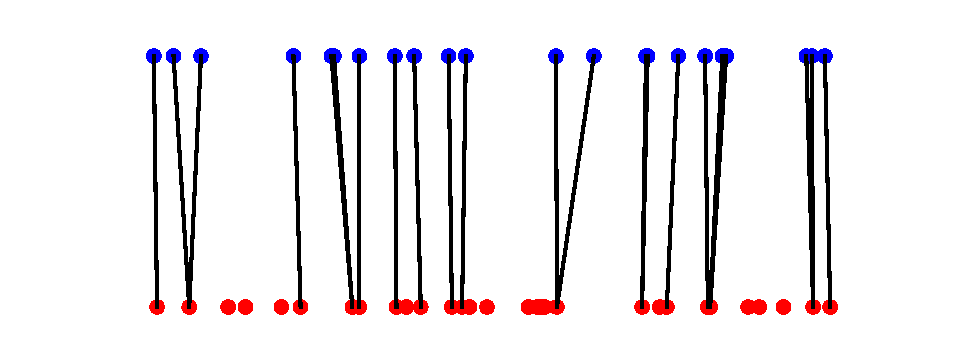
\includegraphics[width = \columnwidth]{t_fig.pdf}
\caption{Nearest Neighbor Assignment}\label{t_fig}
\end{figure}

\begin{figure}[H]
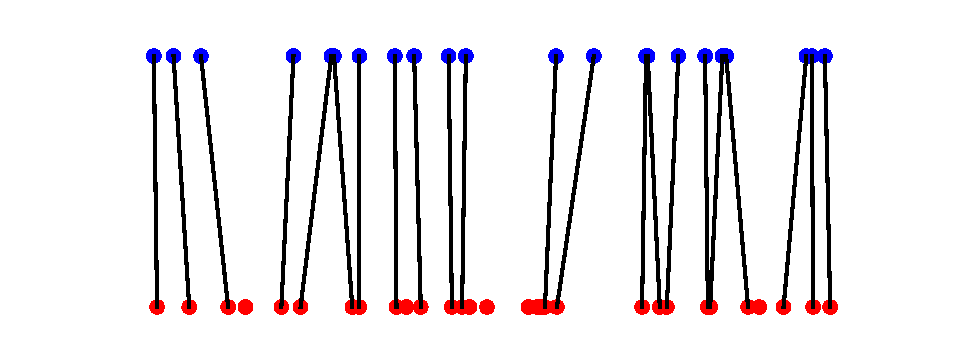
\includegraphics[width = \columnwidth]{a_fig.pdf}
\caption{Partial Optimal Assignment}\label{a_fig}
\end{figure}

Surprisingly, after performances analysis, Numba accelerates loops and succeed in making the quadratic assignment linear with $n$ for $n$ not too big. This is better than expected, and problem decomposition may not be necessary for $n$ smaller than one million. However it could still enables loop parallelization, and reduce complexity for bigger $n$.

\begin{figure}[H]
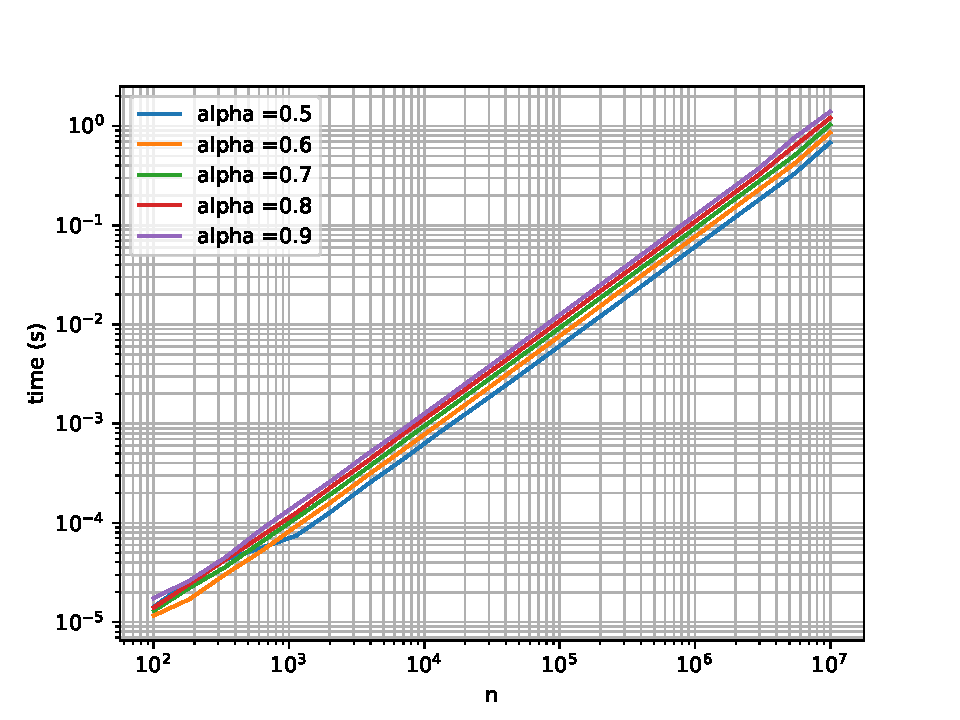
\includegraphics[width = \columnwidth]{a_time.pdf}
\caption{Mean time over $100$ simulations for Quadratic Partial Optimal Assignment with respect to $n$, for different values of $\alpha$, logscale}\label{a_time}
\end{figure}


\subsection{Quasilinear Time Problem Decomposition}

In order to save more computational time, and decrease the complexity of the algorithm Bonneel et al. \cite{BC19} proposed an algorithm to decompose the original problem into many easier subproblems, which can be solved independently with the previous partial optimal assignment algorithm. By doing this, it is possible to parallelize each subproblem solving and gain a consequent amount of time. However, Numba \cite{Numba} the Python library for fast calculation I used, encounters problems with efficient parallelization and I wasn't able to parallelize problem solving after subproblem decomposition. An efficient implementation would require either to debug the Numba library, or to re-implement everything in a compiled language as C\texttt{++}.

The pseudo-algorithm provided by Bonneel et al. seemed to be false (or full of typo), and easy examples where it doesn't work are easy to find. (For example on their Fig. 3, $f_{s_2}$ and $f_{s_3}$ are True so problems $Y_2$ and $Y_3$ are not supposed to merge). I hence took the liberty to rewrite it differently.

The main intuition to the decomposition algorithm is that when considering a new point assignment, we need to either create a new subproblem (if $t[i+1]>a[i]$), or increase the size of the current problem. When increasing the size of the current problem, it is important to note that we just need to consider one more point on the right (case where $a[i+1] = a[i]+1$) and one more point on the left (case where $a[i+1]=a[i]$ and translation). 

Specifically, we again consider an increasing sub-problem involving $\{x_i\}_{i \in \llbracket 1;m' \rrbracket}$ and keep track of the last available free spot $s$ as well as the currently last value $l$ considered by each subproblem. The sub-problem $A_k$ thus involves $\{y_j\}_{j \in \llbracket s_k+1;l_k \rrbracket}$ . We also store a flag $\{f_j\}_{j \in \llbracket 1;n \rrbracket}$ where $f_j$ = false indicates that $y_j$ has been considered by a subproblem at some point in the algorithm, or $f_j$ = true otherwise. \\

\begin{algorithm}
\caption{Decomposition of the assignment problem}\label{subproblem}
\hspace*{\algorithmicindent} \textbf{Input:} sorted $X,Y$\\
\hspace*{\algorithmicindent} \textbf{Output:} $A$ 
\begin{algorithmic}[1]
\State compute $t$
\State initialize Boolean flags $\{f_j\}_{j \in \llbracket 1;n \rrbracket}$ to true;
\For{$m'$ from $1$ to $m$}
	\If{$f_{t[m']}$ is True} \Comment{create new subproblem}
		\State create new subproblem $A_k = (\{x_{m'}\},\{y_{t[m']}\})$	
		\State $f_{t[m']} \gets $ False
    \Else
        \State Consider $A_{k'}$ last subproblem
        \If {$t[m'] \neq t[m'-1]$} \Comment{expand on the right only}
        	\State $A_{k'} \gets (X_{k'} \cup \{x_{m'}\}, Y_{k'} \cup \{y_{l_{k'}+1}\})$
        \Else \Comment{expand on the right and on the left}
        	\While {$f_{s_{k'}}$ is false} \Comment{merge with previous subproblems}
        		\State Consider $A_{k'-1}$ subproblem before $A_{k'}$
        		\State $A_{k'-1} \gets A_{k'} \cup A_{k'-1} = (X_{k'-1} \cup X_{k'},Y_{k'-1} \cup Y_{k'})$
        		\State $k' \gets k'-1$ 
        	\EndWhile
        	\State $A_{k'} \gets (X_{k'} \cup \{x_{m'}\},Y_{k'} \cup \{y_{s_{k'}},y_{l_{k'}+1}\})$
        \EndIf
    \EndIf
\EndFor
\State \Return{$A$}
\end{algorithmic}
\end{algorithm}

It is important to note that the algorithm use the fact that $X$ and $Y$ are sorted, and is hence made in such a way that consecutive subproblems $A_k$ and $A_{k+1}$ consider consecutive values of $X$ and increasing values of $Y$, which means that $l_k \leqslant s_{k+1}$.

\begin{figure}[H]
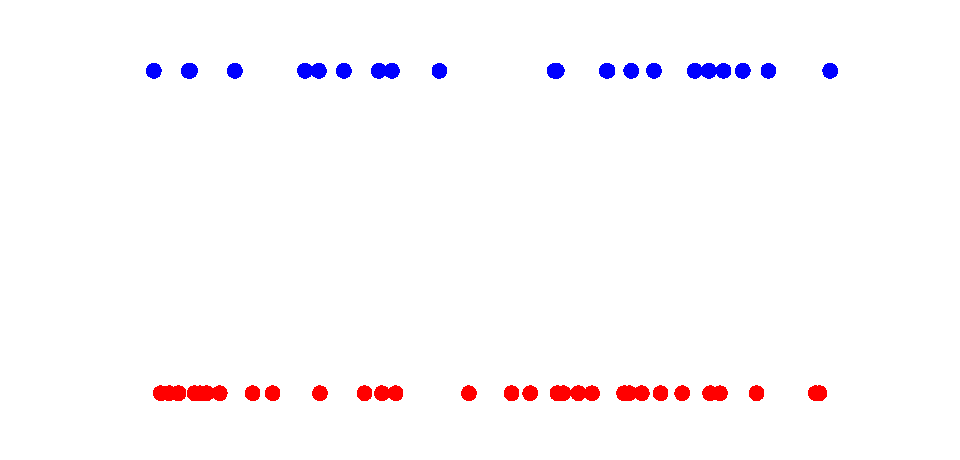
\includegraphics[width = \columnwidth]{before_decomp.pdf}
\begin{center}
$\downarrow$
\end{center}
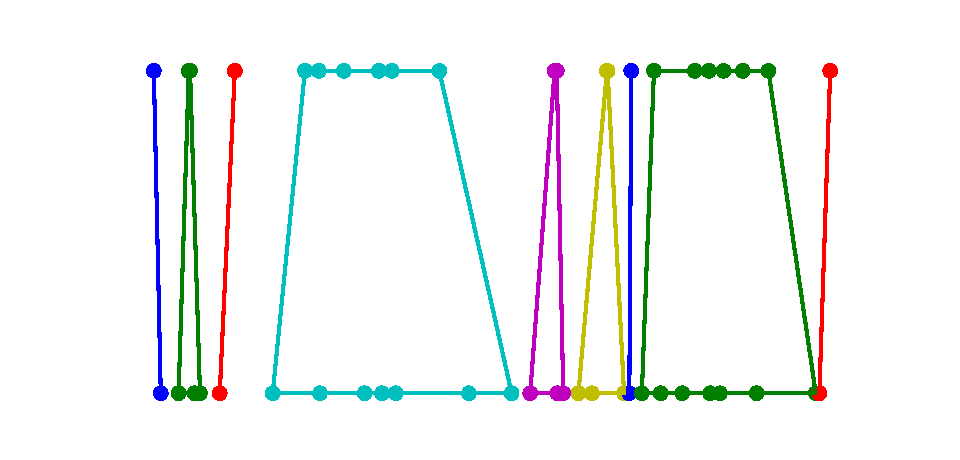
\includegraphics[width = \columnwidth]{decomp_fig.pdf}
\caption{Assignment problem decomposition}\label{decomp_fig}
\end{figure}

\begin{figure}[H]
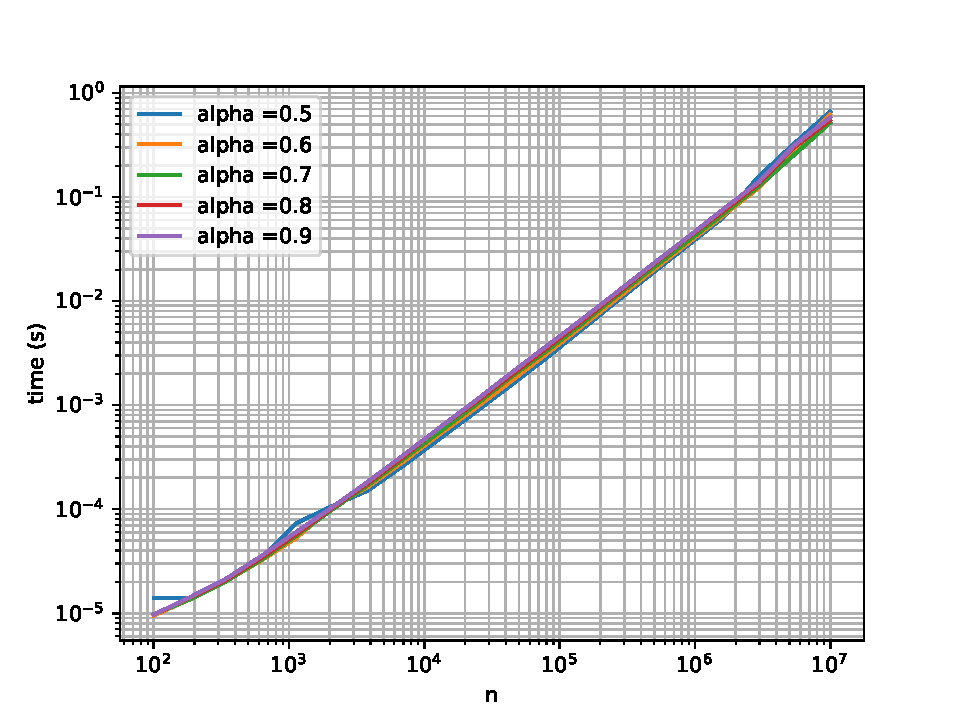
\includegraphics[width = \columnwidth]{decomp_time.pdf}
\caption{Mean time over $100$ simulations for the decomposition of the assignment problem with respect to $n$, for different values of $\alpha$, logscale}\label{decomp_time}
\end{figure}


\section{Sliced Partial Transport}

While 1-d optimal transport has limited interest per se, it is the main ingredient of sliced optimal transport. Sliced optimal transport is a very fast algorithm that shares similar properties with optimal transport and works in n dimensions.

The partial 1-d optimal transport solution provided in the last section, while of quadratic complexity in the worst case, is fast (see Fig. \ref{t_time}, \ref{a_time}, \ref{a_time_decomp}) and is thus amenable to the computation of sliced optimal transport.

In the sliced framework, instead of minimizing directly the n-dimensional Wasserstein distance, we minimize the mean over all one-dimensional subspaces of the one-dimensional Wasserstein distance between the one-dimensional projections of the point sets :

\begin{equation}
\min_{\tilde{X}} \int_{S^{d-1}} W_S(Proj_\omega(\tilde{X}),Proj_\omega(Y))\,d\omega
\end{equation}

\noindent where $S^{d−1}$ is the (d-1)-dimensional sphere of directions.

To do so, we use a classical gradient descent with mini-batch size of one. We start by initializing $X_0 = X$. Then, at each iteration $k$, we choose a random direction $\omega$ and compute the gradient of $E_\omega(X_k) = W_S(Proj_\omega(X_k),Proj_\omega(Y))$ which is :

\begin{equation}
\nabla_{X}  E_\omega(X_k) = Proj_\omega(X_k)-Proj_\omega(Y \circ a)
\end{equation}

\noindent where $a$ is the optimal partial assignment between $Proj_\omega(\tilde{X})$ and $Proj_\omega(Y)$. 

We update $X_k$ with the step:

$$
X_{k+1} = X_k - \eta_k \nabla_{X}  E_\omega(X_k)
$$

\noindent With $\eta_k>0$ the learning rate. Formally, in order to be sure of the algorithm convergence, $\eta_k$ must be chosen such as $\sum_{k=0}^{+\infty} \eta_k = +\infty$ and $\sum_{k=0}^{+\infty} \eta_k^2 < +\infty$. In fact, this algorithm works well with a constant learning rate in some cases.

At the end of the algorithm, we get $X^*$ an approximation of the optimal partial assignment of $X$ to $Y$.


\section{Results}

\subsection{Color Transfer}

Once all the previous method has been implemented, color transfer is easy to do : The algorithm is just a gradient descent described as above, with sliced partial optimal transport, and a learning step $\eta$ constant equal to 1. The use of sliced partial optimal transport makes it possible to transfer color from images of different sizes. But the interesting point about that, is that it makes it possible to do a good color transfer between images that have not their content not in the same proportion. 

For example in Fig. \ref{42_fig} and \ref{41_fig}, the input image has a lot more trees than the target image. As a consequence, if no upscaling of the target image is done, trees takes the blue color of the sky.

\begin{figure}[H]
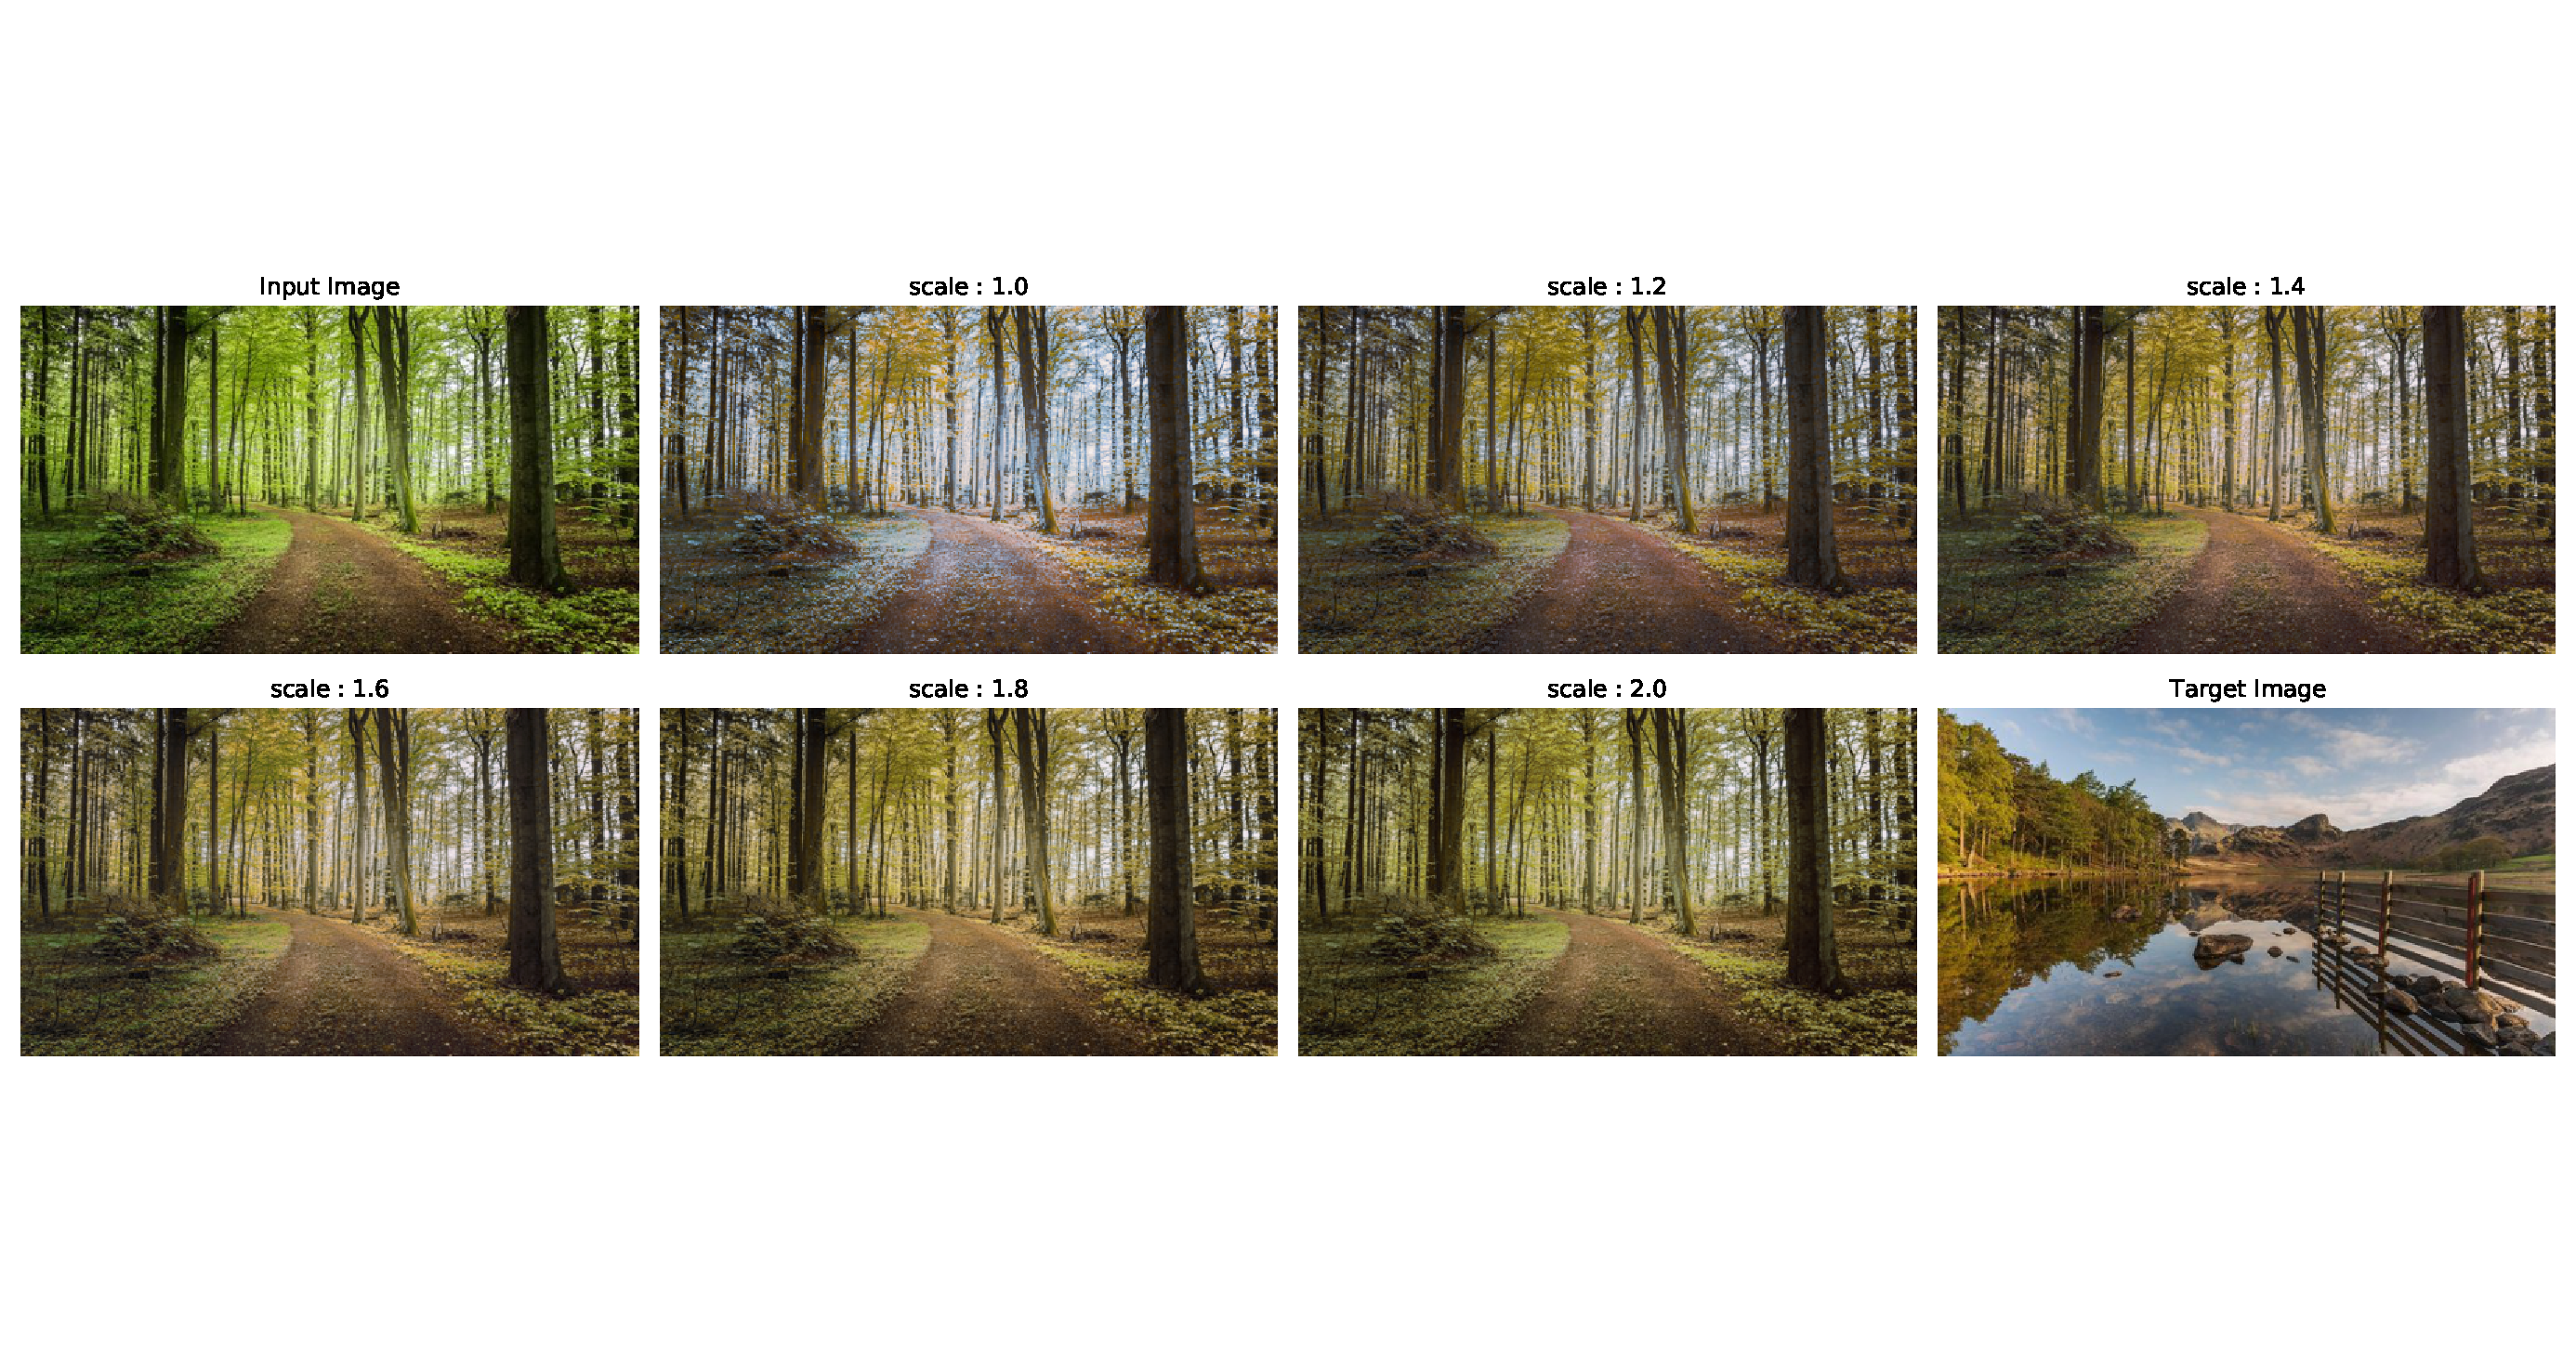
\includegraphics[trim=0cm 3cm 0cm 1.5cm, width = \columnwidth]{landscape42.pdf}
\caption{Color transfer between images using sliced partial optimal transport, input image has more trees}\label{42_fig}
\end{figure}

\begin{figure}[H]
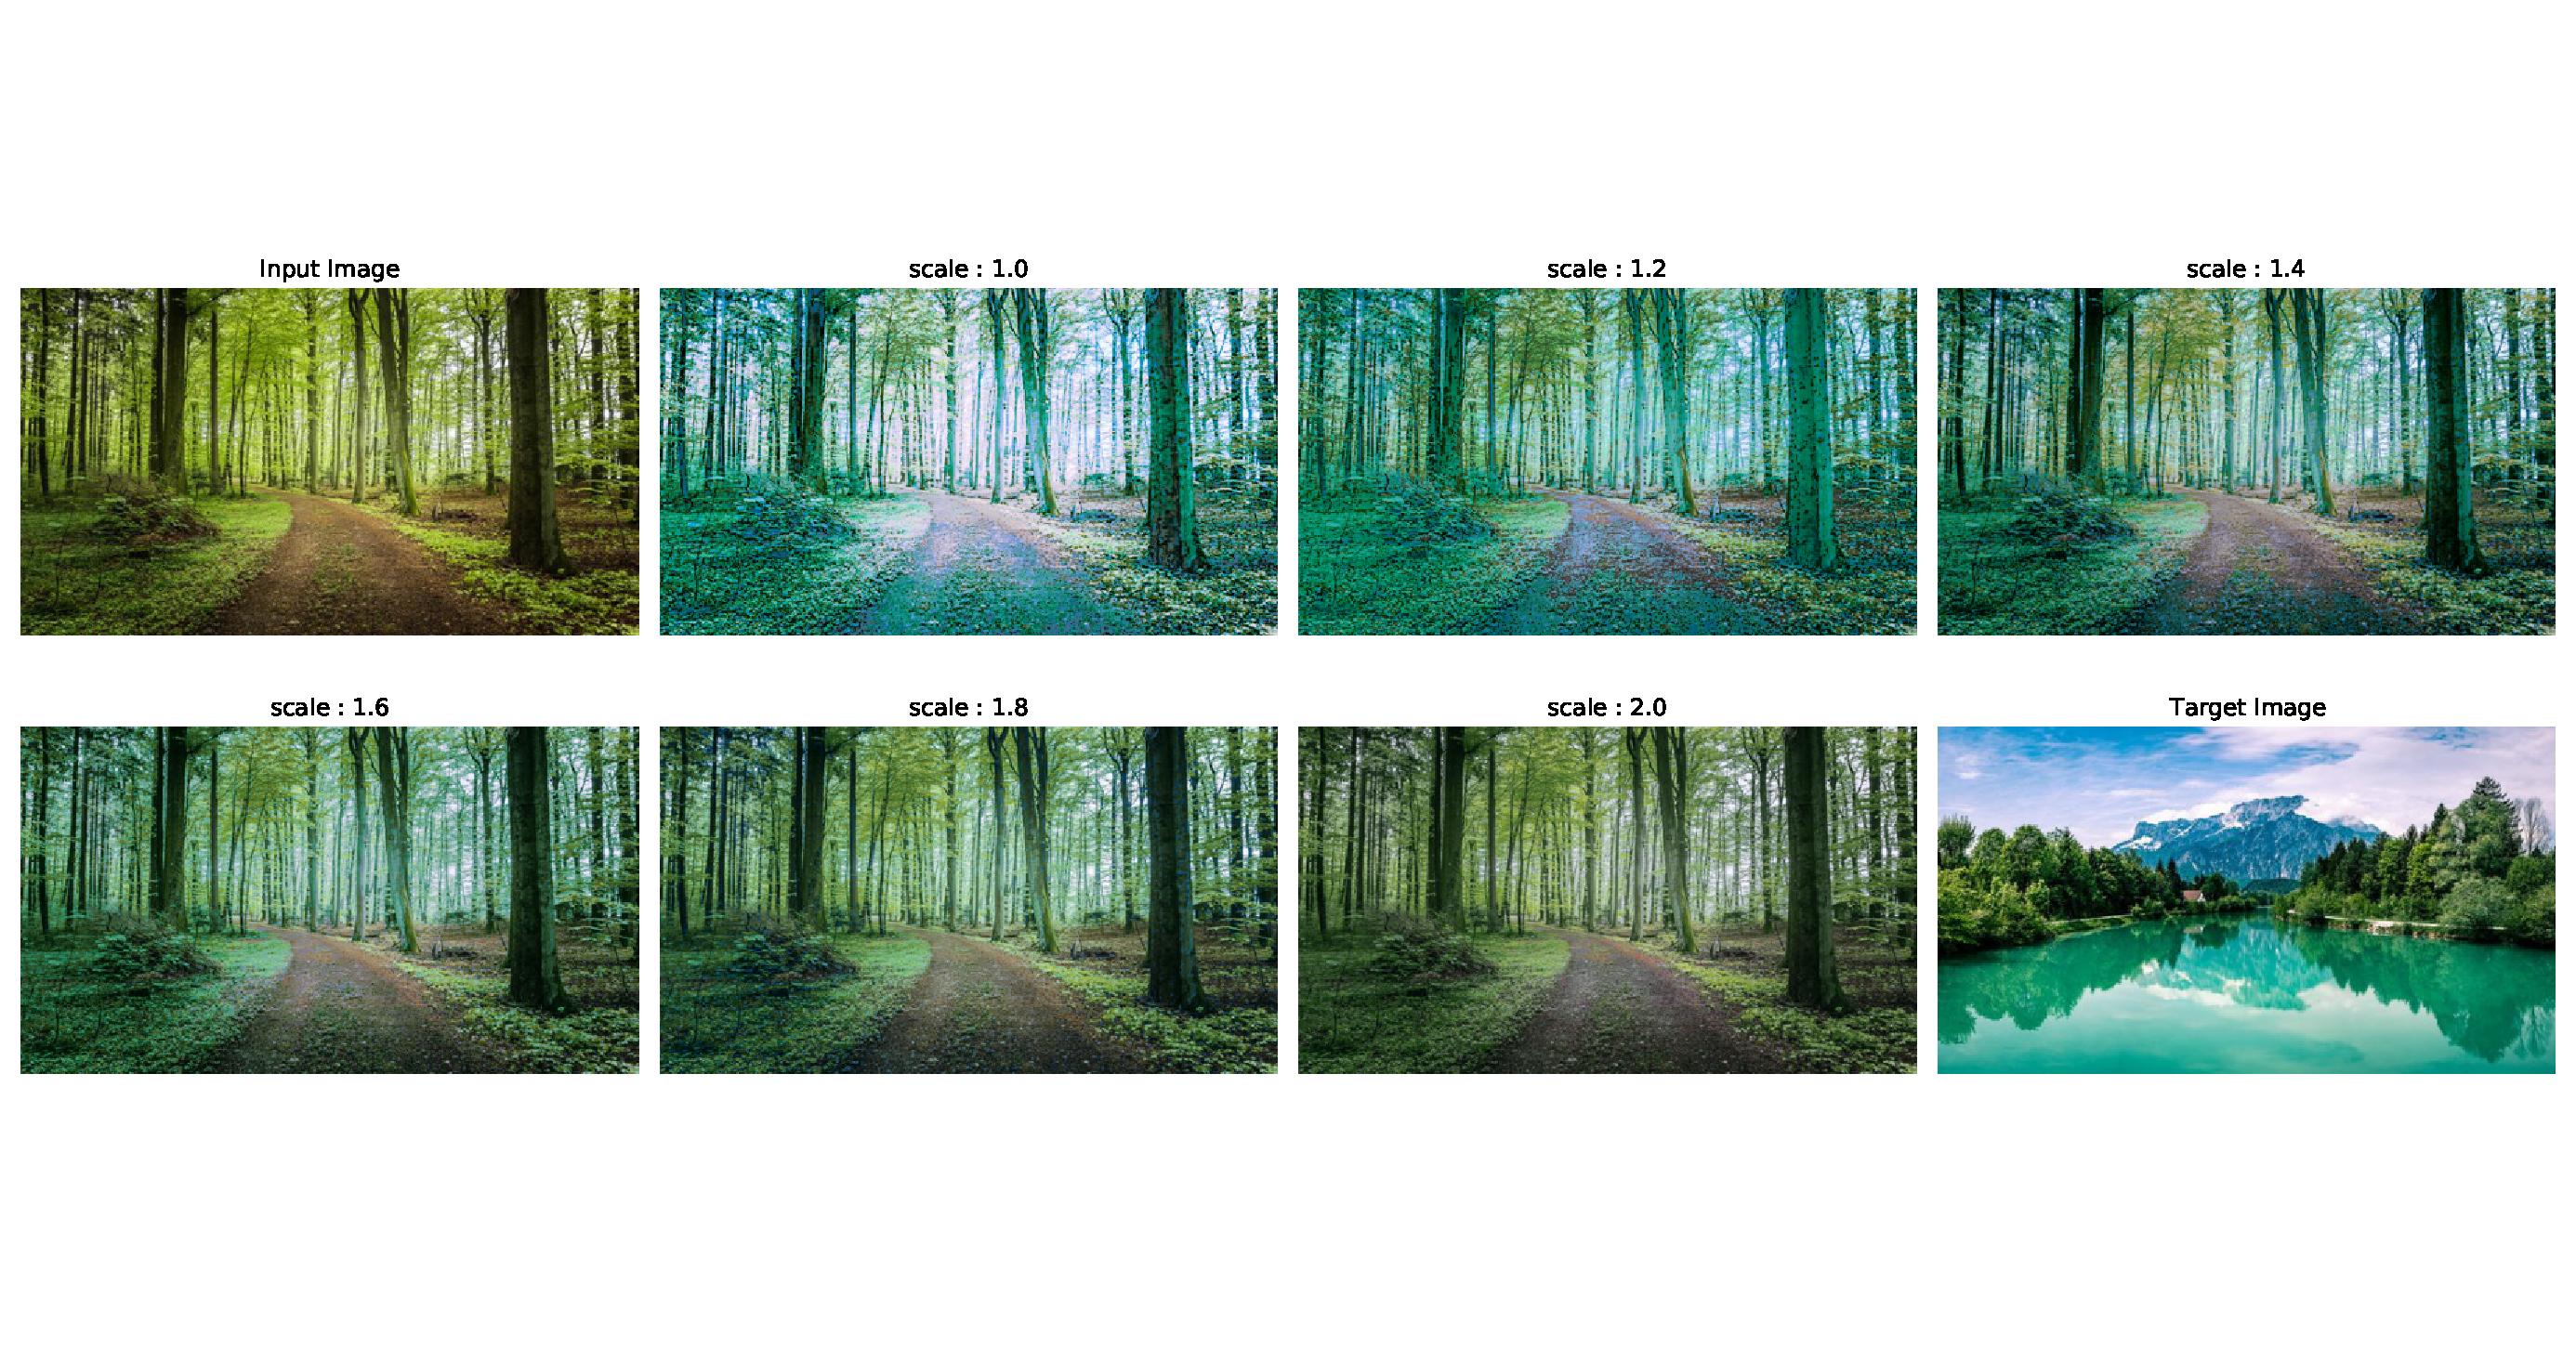
\includegraphics[trim=0cm 3cm 0cm 1.5cm, width = \columnwidth]{landscape41.pdf}
\caption{Color transfer between images using sliced partial optimal transport, input image has more trees and is bluer}\label{41_fig}
\end{figure}

In the same way, in Fig. \ref{21_fig}, the target image has too much blue, and if no upscaling is done, almost the entire output image is blue.

\begin{figure}[H]
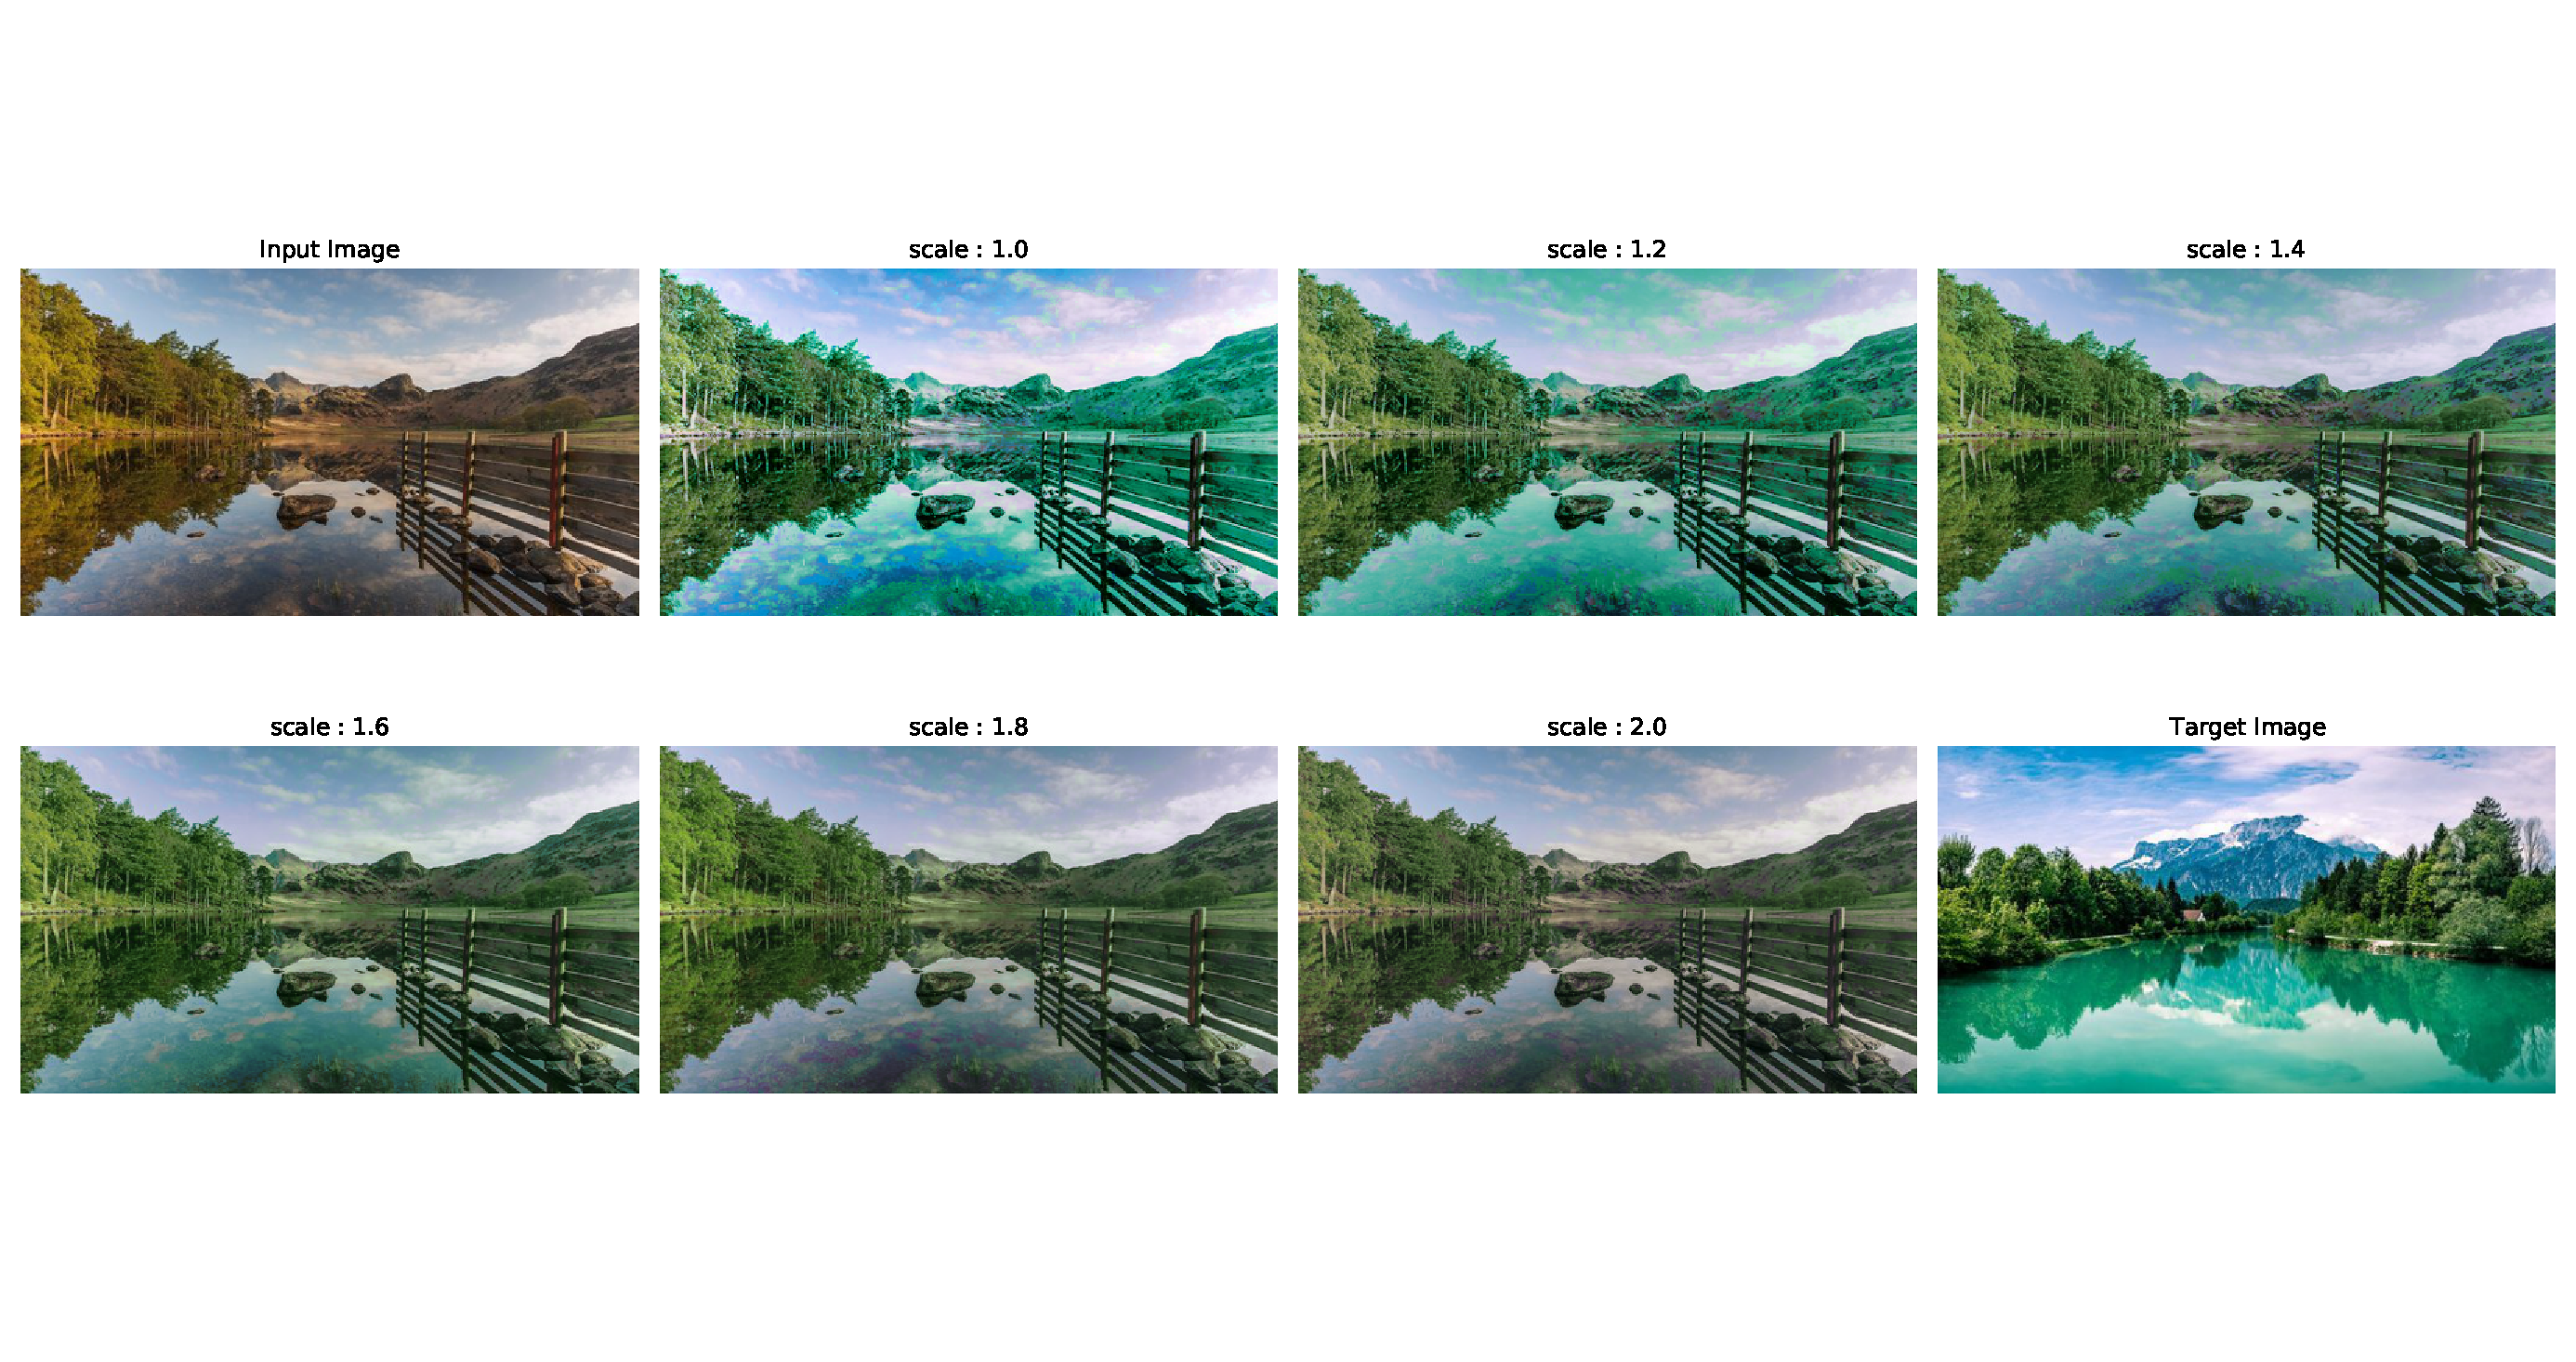
\includegraphics[trim=0cm 3cm 0cm 1.5cm, width = \columnwidth]{landscape21.pdf}
\caption{Color transfer between images using sliced partial optimal transport, input image is bluer}\label{21_fig}
\end{figure}

However, doing too much upscaling can result in a bad output image. This can be seen in the Fig. \ref{12_fig}, where a scale foactor of 1.1 or 1.2 seems better than 1.5, where the trees have taken the color of the mountains of the target image.

\begin{figure}[H]
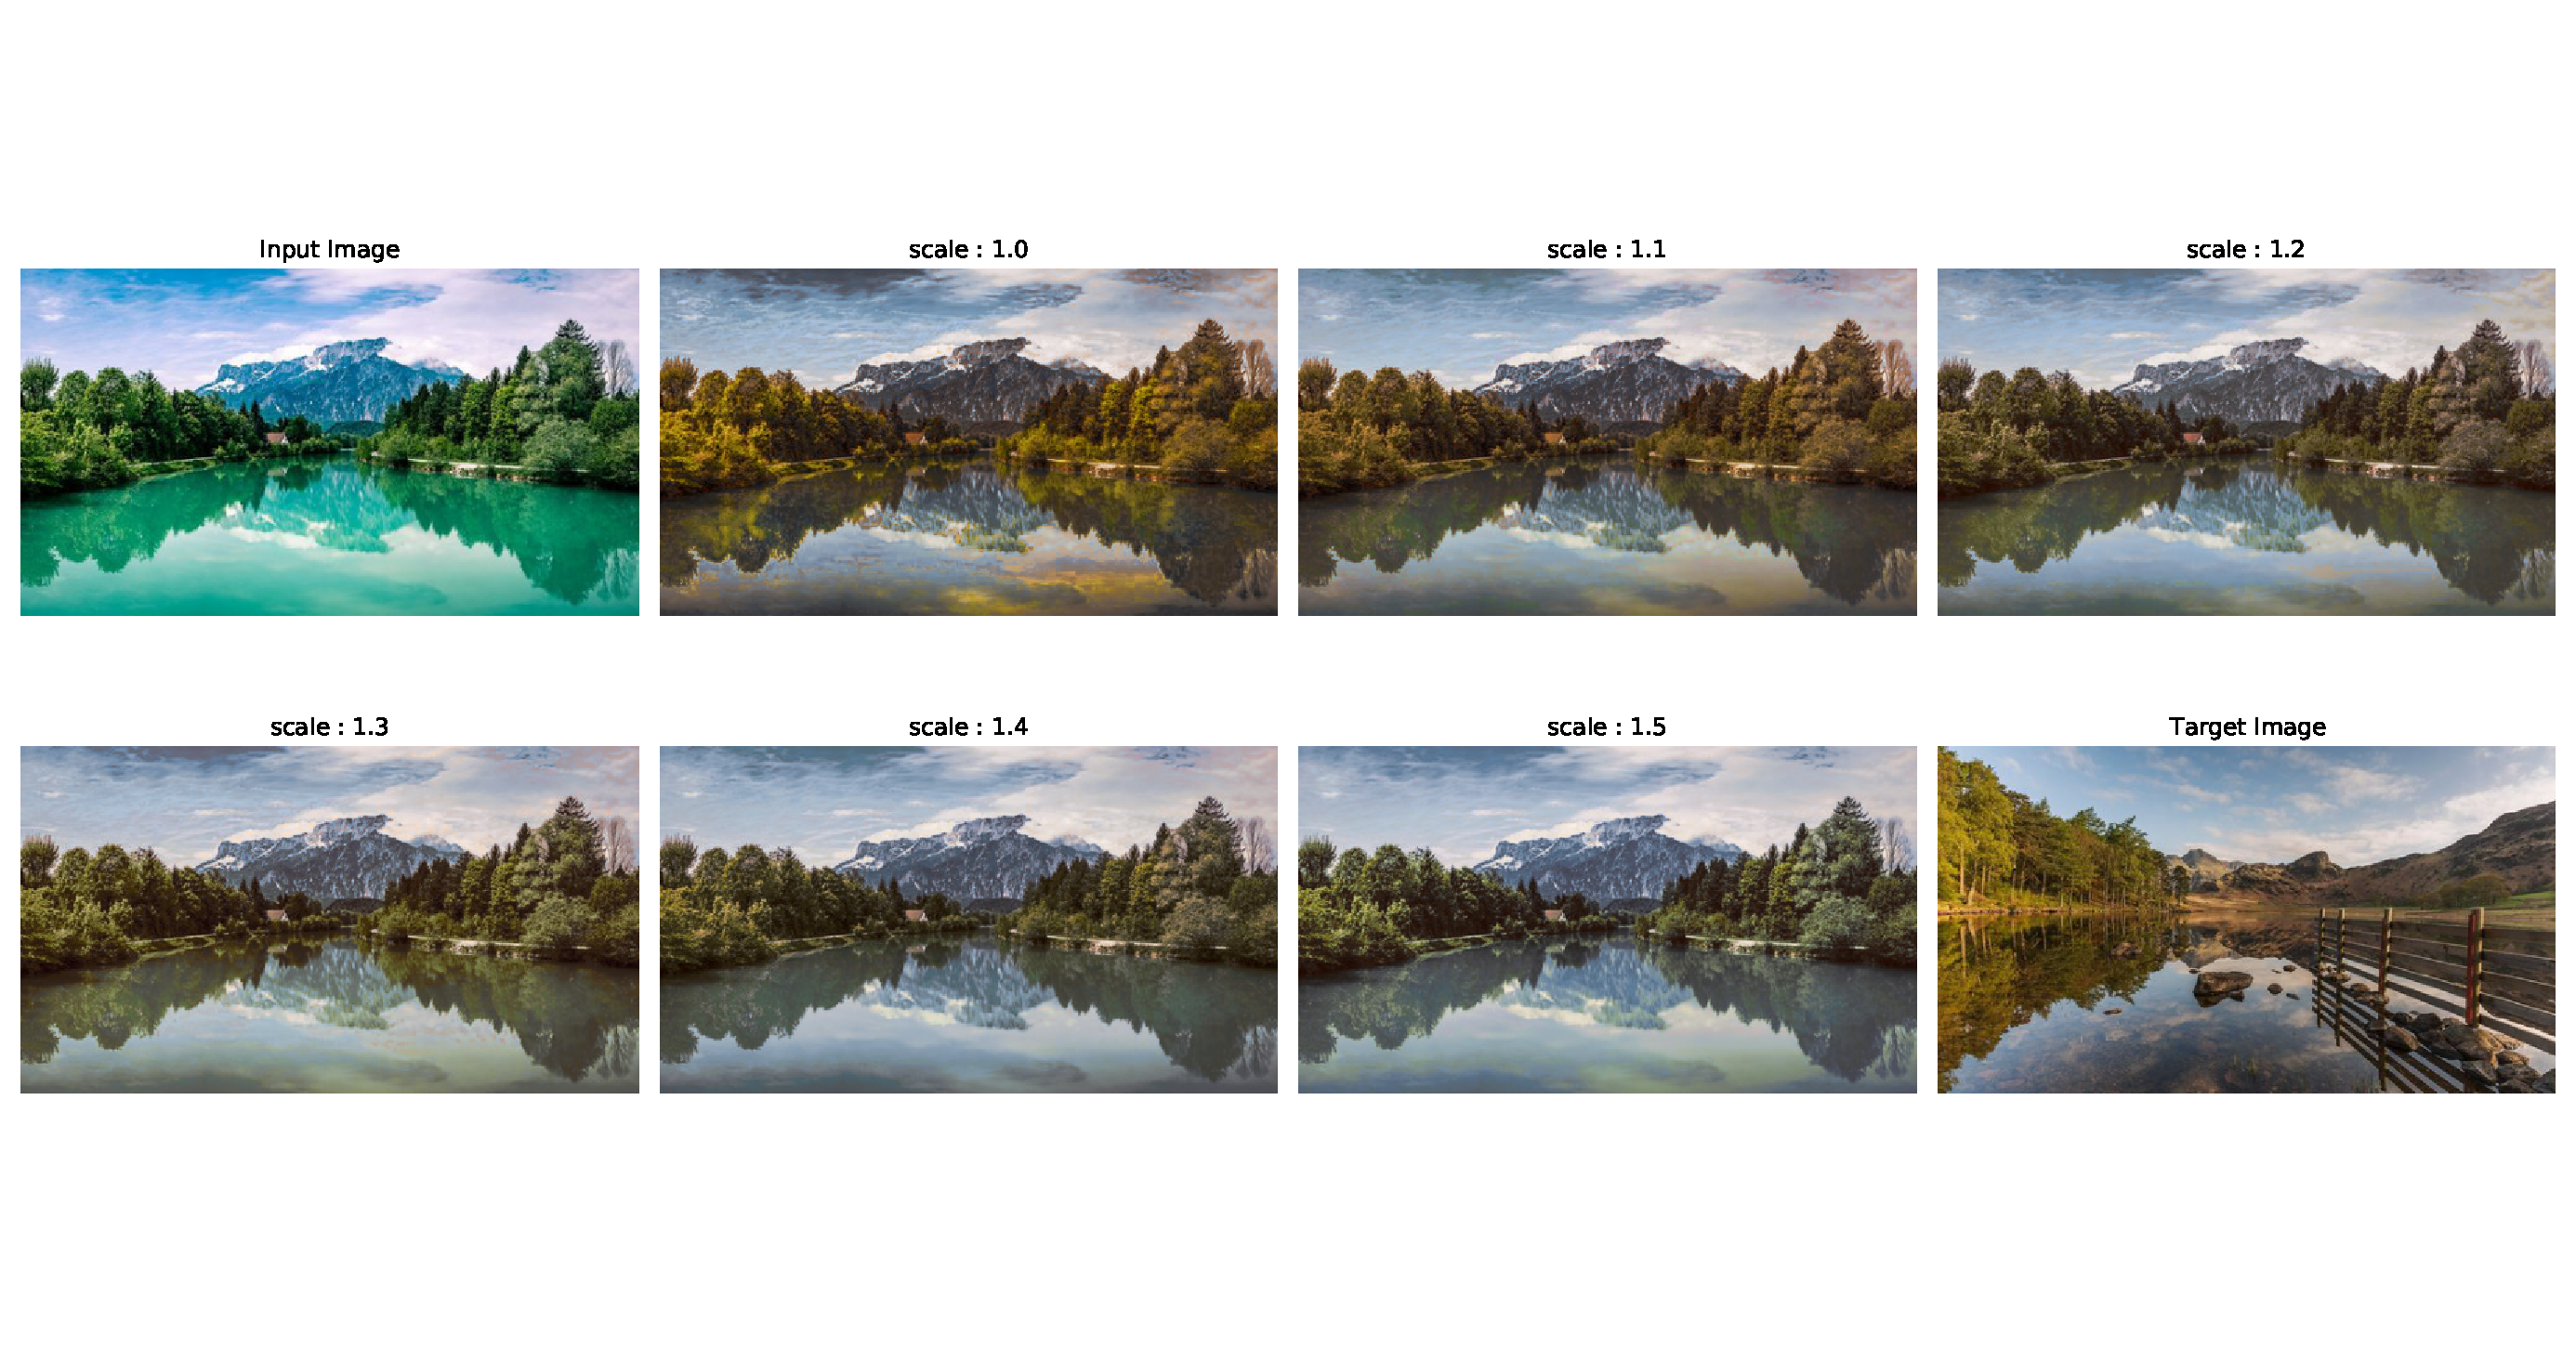
\includegraphics[trim=0cm 3cm 0cm 1.5cm, width = \columnwidth]{landscape12.pdf}
\caption{Color transfer between images using sliced partial optimal transport, input and target images have the same content}\label{12_fig}
\end{figure}

Every simulations were done with images of size $500 \times 281$ pixels, and with 300 iterations. It took between 1 and 5 minutes (depending on the scale factor) to run.

\subsection{Point Cloud Registration}

Point Cloud registration required a different method which is variation of the Iterative Closest Point Algorithm : the FIST. As stated in the introduction, this algorithm consists in doing a sliced optimal transport in one-dimension, then finding the best similarity transformation to match the transformation described by the partial assignment, and finally update the point cloud with this transformation. To find the best similarity transformation, we solve the Orthogonal Procrustes problem \cite{schonemann1966generalized}, to find the best rotation between the centered point cloud and its centered assignment, we scale it and recenter it, so it has the same scale and center as its assignment in the target point cloud.

\begin{figure}[H]
\centering
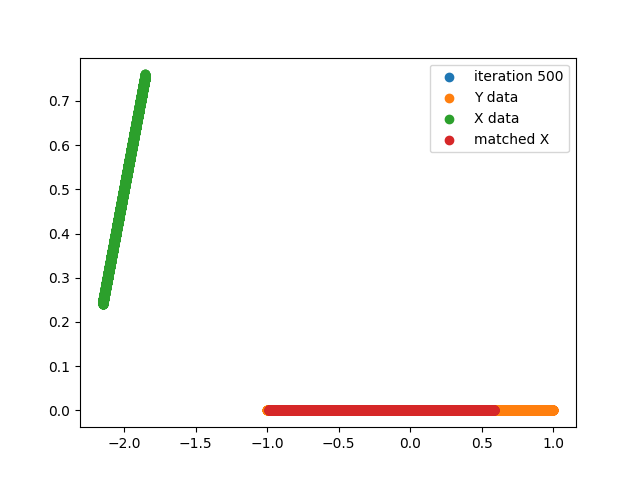
\includegraphics[scale = 0.45]{line_shape.png}
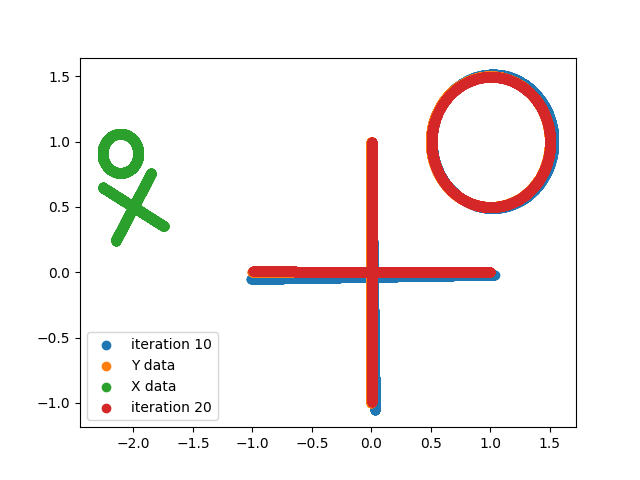
\includegraphics[scale = 0.45]{circle_cross_shape.png}
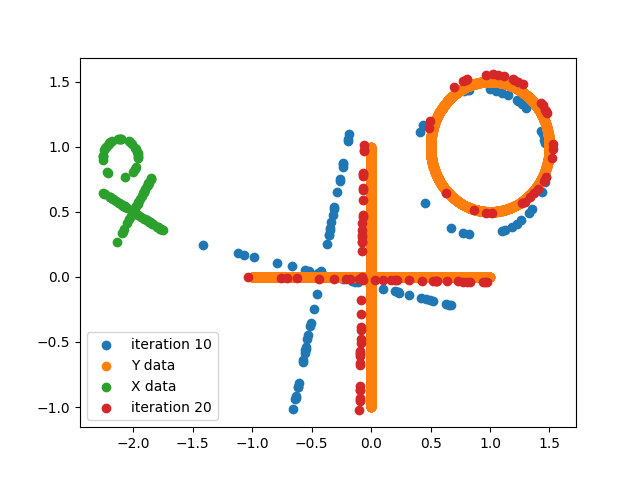
\includegraphics[scale = 0.45]{circle_cross_shape2.png}
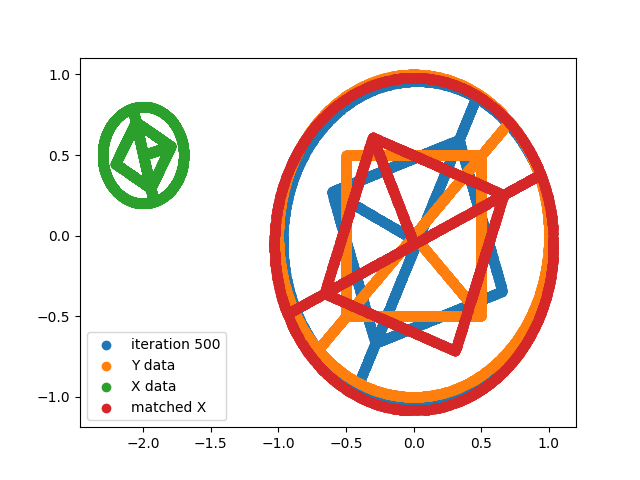
\includegraphics[scale = 0.45]{circle_shape.png}
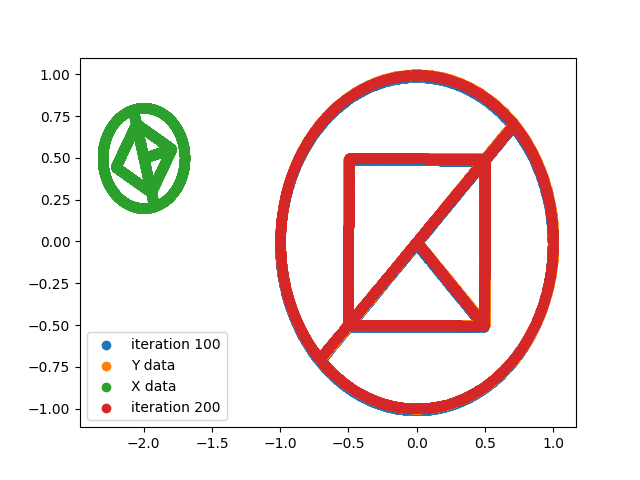
\includegraphics[scale = 0.45]{circle_shape2.png}
\caption{Point cloud Registration for different shapes}\label{shape}
\end{figure}

Results are impressive for shapes that have not too much symmetries. For example, for the shape with the cross and the circle, there is convergence with 20 iterations, even with only 1\% of the points. However, there is never convergence with the line, no matter the number of iterations. Finally with the last shape, which is more complex, there is always convergence, but sometimes to a local minimum, and it requires at least 200 iterations to converge.

In the figure \ref{shape}, the target point cloud is of size 10 000, and the input point cloud is of size 8 000, except for the third figure where the input cloud is of size 100. it takes approximately one second for 50 iterations and input and target point clouds respectively of size 10 000 and 8 000.

\section{Appendix}

\subsection{Proof of the optimality of algorithm \ref{a_quad}}
\label{a_quad_proof}

\noindent \underline{By mathematical induction}:\\
Let $n \in \mathbb{N}$.
Let $t$ be the nearest neighbor assignment from $X$ to $Y$.
Let $P(m)$ be the property : algorithm \ref{a_quad} gives the optimal assignment for $card(X)=m$ and $card(Y)=n$.\\
\noindent \underline{Initial step}: It is trivial for $m$=1 \\
\noindent \underline{Inductive Step}: Assume that $P(m)$ is true. We want to show that $P(m+1)$ is true. \\
\noindent Tanks to $P(m)$, we have $a_m : \llbracket 1;m \rrbracket \rightarrow \llbracket 1;n \rrbracket$ the optimal partial assignment from $\{x_i\}_{i \in \llbracket 1;m \rrbracket}$ to $Y$.\\
\noindent If $a_m[m] < t[m+1]$, then $a_{m+1}$ such that $a_{m+1}(i)=a_m(i)$ if $i \leqslant m$ and $a_{m+1}(m+1)=t(m+1)$ is clearly optimal.\\
\noindent
\noindent If $t[m+1] \leqslant a_m[m]$, then, $x_{m+1}$ cannot be optimally assigned to any $y_l$ with $l>a_m[m]+1$. Indeed, as the nearest neighbor of $x_{m+1}$ is (strictly) before $y_{a_m[m]+1}$, any other assignment of $x_{m+1}$ would have a higher cost. \\
\noindent Moreover, an optimal 1-D assignment $a$ has no intersections. That means that there is no $x_i < x_j$ such that $y_{a[j]} < y_{a[i]}$. Therefore $x_{m+1}$  cannot be assigned to $y_l$ with $l<a_m[m]$, and if $x_{m+1}$ is assigned to $y_{a_m[m]}$, then $a_{m+1}[r:m] = a_{m}[r:m]-1$.\\
\noindent As a consequence, is only two cases left, which are the case one and the case 2 of the algorithm. The optimal partial assignment $a_{m+1}$ is that which has the smaller cost between case 1 and case 2.
\noindent Therefore $a_{m+1}$ as described by the algorithm is optimal.\\
\noindent \underline{Conclusion}: $P(m)$ is true for $m \in \llbracket 1;n \rrbracket$. Therefore algorithm \ref{a_quad} is optimal for all $n \in \mathbb{N}$ and for all $m \in \llbracket 1;n \rrbracket$.

\bigskip

\addsec{Conclusion}
%\section*{Conclusion}

To Summarize, in this project I have :
\begin{itemize}
\item Made a fast python implementation of Sliced Partial Optimal Transport. This method is fast and efficient in time and memory. I have implemented the problem decomposition but I am not able to parallelize it easily because of a bug in the numba library. To overcome this problem, one should either implement it in Cexttt{++}, debug numba, or use cython instead of numba.
\item Implemented a color transfer method that works with images that have content with different proportions. It works well and it is fast. However it is not always better to upscale the target image, as it can lead to a faded image.
\item Implemented the FIST algorithm for point cloud registration. It is a really fast method for matching point clouds. I have tested it in 2D but not in 3D, even though it would be easy to do. This method could be improved by adding a way not to stay in a local minimum.
\end{itemize}




\bibliographystyle{unsrt}
\bibliography{bibli}

\end{document}
